\iffalse
\documentclass[12pt]{article}
\usepackage{graphicx}
\usepackage{amsmath}
\usepackage{mathtools}
\usepackage{gensymb}

\newcommand{\mydet}[1]{\ensuremath{\begin{vmatrix}#1\end{vmatrix}}}
\providecommand{\brak}[1]{\ensuremath{\left(#1\right)}}
\providecommand{\norm}[1]{\left\lVert#1\right\rVert}
\newcommand{\solution}{\noindent \textbf{Solution: }}
\newcommand{\myvec}[1]{\ensuremath{\begin{pmatrix}#1\end{pmatrix}}}
\let\vec\mathbf

\begin{document}
\begin{center}
\textbf\large{CHAPTER-7 \\ COORDINATE GEOMETRY}

\end{center}
\section*{Excercise 7.4}

Q4.The two opposite vertices of a square are $(–1, 2) \text{ and } (3, 2)$. Find the coordinates of the other two vertices.\\
\fi
\solution
Let
\begin{align}
\vec{A} = \myvec
{
-1 \\
 2\\
},
\vec{C} = 
\myvec
{
3\\
2\\
}
\end{align}

\begin{figure}[!h]
	\begin{center} 
	    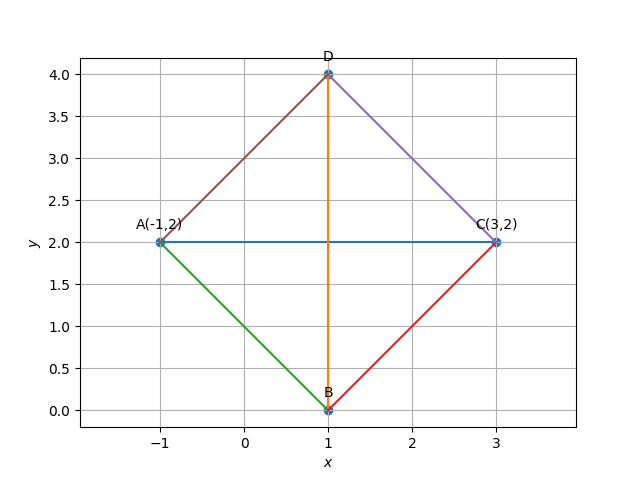
\includegraphics[width=\columnwidth]{chapters/10/7/4/4/figs/square}
	\end{center}
\caption{}
\label{fig:7/4/4/4Fig1}
\end{figure}

Shifting $\vec{A}$ to origin with reference to Fig. \ref{fig:7/4/4/4Fig2},
\begin{align}
\vec{A^{\prime}} =
\myvec{
0 \\
0\\
},
\vec{C^{\prime}} = \vec{C}-\vec{A} = 
\myvec{
4 \\
0\\
}
\end{align}

\begin{figure}[!h]
	\begin{center} 
	    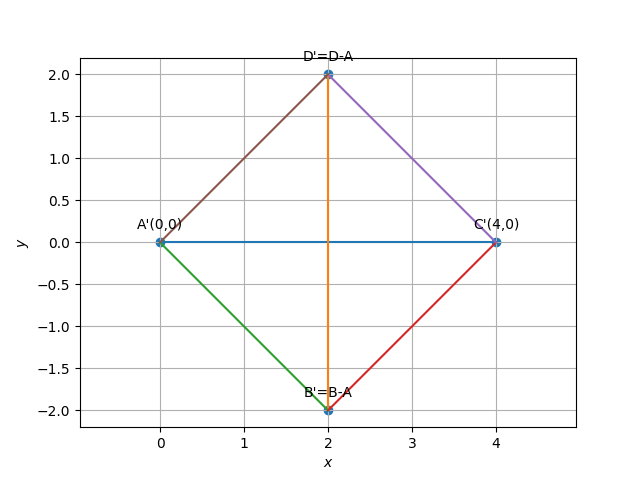
\includegraphics[width=\columnwidth]{chapters/10/7/4/4/figs/square1}
	\end{center}
\caption{}
\label{fig:7/4/4/4Fig2}
\end{figure}
\iffalse
In general,
the angle made by $AC$ with the x-axis is 
		\begin{align}
\beta = \theta + 45\degree
		\end{align}
\fi
Since
\begin{align}
\vec{C} - \vec{A} = \myvec{
4\\
0
} \equiv 
\myvec{
1\\
0
},
	\tan\theta&= \frac{0}{4} \implies 
\theta= 0\degree
\end{align}
		where
$\theta$ is the angle made by $AC$ with the x-axis.
Considering the rotation matrix 
\begin{align}
\vec{P} =
\myvec{
\cos\brak{\frac{\pi}{4}-\theta} & -\sin\brak{\frac{\pi}{4}-\theta} \\
\sin\brak{\frac{\pi}{4}-\theta} & \cos\brak{\frac{\pi}{4}-\theta} 
}
\end{align}
\iffalse
from Fig. \ref{fig:7/4/4/4Fig3},
\begin{align}
\vec{C^{\prime \prime}} = \vec{P}^\top (\vec{C}-\vec{A}) =
\myvec{
\frac{1}{\sqrt{2}} & -\frac{1}{\sqrt{2}} \\
\frac{1}{\sqrt{2}} & \frac{1}{\sqrt{2}}\\
}
\myvec{
4 \\
0\\
} = 
\myvec{
\frac{4}{\sqrt{2}} \\
\frac{4}{\sqrt{2}}\\
}
\end{align}
\begin{align}
\vec{B^{\prime \prime}} = \myvec{
 1&0\\
 0&0\\
}\vec{C^{\prime \prime}}=
\myvec{
 \frac{4}{\sqrt{2}}\\
 0\\
},
\vec{D^{\prime \prime}} = \myvec{
 0&0\\
 0&1\\
}\vec{C^{\prime \prime}}=
\myvec{
 0\\
 \frac{4}{\sqrt{2}}\\
} \text{ and }
\vec{A^{\prime \prime}} =
\myvec{
0 \\
0\\
}
\end{align}
\fi
\begin{figure}[!h]
	\begin{center} 
	    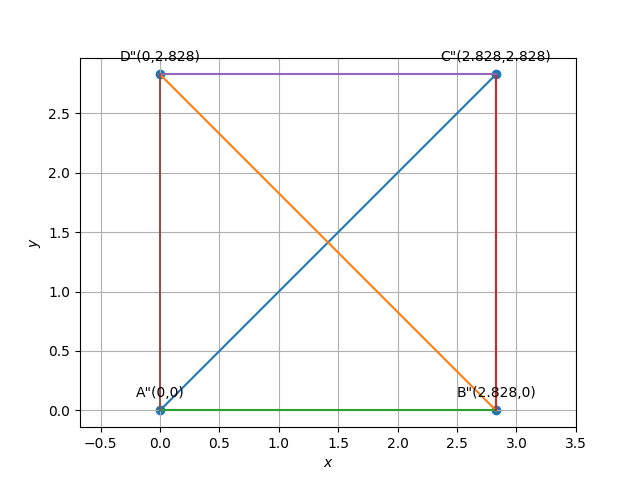
\includegraphics[width=\columnwidth]{chapters/10/7/4/4/figs/square2}
	\end{center}
\caption{}
\label{fig:7/4/4/4Fig3}
\end{figure}

\newpage
\iffalse
Again tranforming(rotating) the coordinates back to the original axis.

We know for anti-clockwise direction the rotation matrix is given as
\begin{align}
\vec{P} =
\myvec{
\cos\theta & -\sin\theta \\
\sin\theta & \cos\theta \\
}
\end{align}

Again we know that the angle is negative so the rotation will be in clockwise direction. So now the transformed(rotated) coordinates $\vec{B} \text{ and } \vec{D}$ are with refrence to 
\fi
from Figure 
%\ref{fig:7/4/4/4Fig4},
\ref{fig:7/4/4/4Fig3},
\begin{align}
	\vec{C^{\prime \prime}} &= \vec{P} (\vec{C}-\vec{A}) 
	\\
\label{eq:7/4/4/4bp}
	\vec{B^{\prime \prime}} &= \myvec{\vec{e}_1 & \vec{0}}\vec{C^{\prime \prime}}
	\\
\label{eq:7/4/4/4dp}
	\vec{D^{\prime \prime}} &= \myvec{ \vec{0} & \vec{e}_2}\vec{C^{\prime \prime}}
\end{align}
Now, 
\begin{align}
\label{eq:7/4/4/4b}
	\vec{B} = \vec{P}^{\top}\vec{B}^{\prime \prime}+\vec{A}
	\\
\label{eq:7/4/4/4d}
	\vec{D} = \vec{P}^{\top}\vec{D}^{\prime \prime}+\vec{A}
\end{align}
by reversing the process of translation and rotation.  Thus, 
from
\eqref{eq:7/4/4/4b}
\eqref{eq:7/4/4/4bp},
\eqref{eq:7/4/4/4d}
and
\eqref{eq:7/4/4/4dp}
\begin{align}
	\vec{B} = \vec{P}^{\top}\myvec{\vec{e}_1 & \vec{0}}\vec{P} (\vec{C}-\vec{A}) +\vec{A}
	\\
	\vec{D} = \vec{P}^{\top}\myvec{\vec{0} & \vec{e}_2  }\vec{P} (\vec{C}-\vec{A}) +\vec{A}
%	\vec{B} &= \brak{(\vec{C}-\vec{A})^{\top}\vec{P}^{\top} \vec{e}_1}\vec{P}^{\top}\vec{e}_1+\vec{A}
%	\\
%	\vec{D} &= \brak{(\vec{C}-\vec{A})^{\top}\vec{P}^{\top} \vec{e}_2}\vec{P}^{\top}\vec{e}_2+\vec{A}
\end{align}
yielding
		\begin{align}
\vec{B}=
\myvec{
1\\
0
},
\vec{D}
\myvec{
1\\
4
}.
		\end{align}
\iffalse
\begin{align}
\vec{B^{\prime}} &= \vec{P}\vec{B^{\prime \prime}} = \myvec{
\frac{1}{\sqrt{2}} & \frac{1}{\sqrt{2}} \\
-\frac{1}{\sqrt{2}} & \frac{1}{\sqrt{2}}\\
}
\myvec{
 \frac{4}{\sqrt{2}}\\
 0\\
} = 
\myvec{
2 \\
-2\\
}\\
\vec{D^{\prime}} &= \vec{P}\vec{D^{\prime \prime}} = \myvec{
\frac{1}{\sqrt{2}} & \frac{1}{\sqrt{2}} \\
-\frac{1}{\sqrt{2}} & \frac{1}{\sqrt{2}}\\
}
\myvec{
 0\\
 \frac{4}{\sqrt{2}}\\
} = 
\myvec{
2 \\
2 \\
}
\end{align}

\begin{figure}[!h]
	\begin{center} 
	    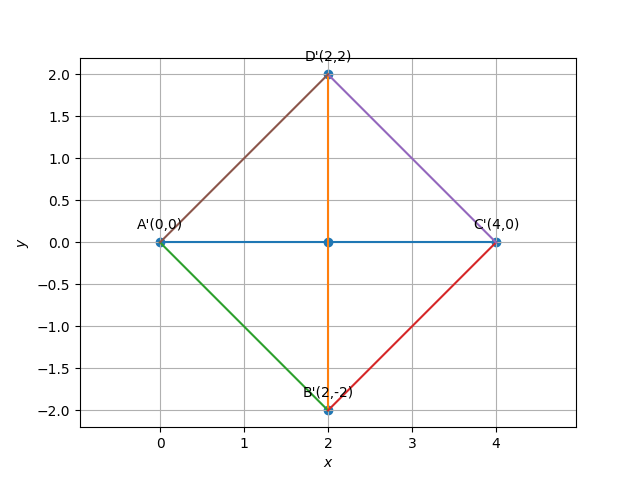
\includegraphics[width=\columnwidth]{chapters/10/7/4/4/figs/square3}
	\end{center}
\caption{}
\label{fig:7/4/4/4Fig4}
\end{figure}

Again transforming(shifting) the axis back to the original with refrence to Figure \ref{fig:7/4/4/4Fig5}
\begin{align}
\vec{B} &= \vec{B^{\prime}}+\vec{A} = \myvec{
2 \\
-2\\
}+\myvec{
-1 \\
2\\
} = 
\myvec{
1 \\
0\\
}\\
\vec{D} &= \vec{D^{\prime}}+\vec{A} = \myvec{
2 \\
2\\
}+\myvec{
-1 \\
2\\
} = 
\myvec{
1 \\
4 \\
}
\end{align}

Hence, the other two vertices are $\vec{B}(1,0) \text{ and } \vec{D}(1,4)$   

\begin{figure}[!h]
	\begin{center} 
	    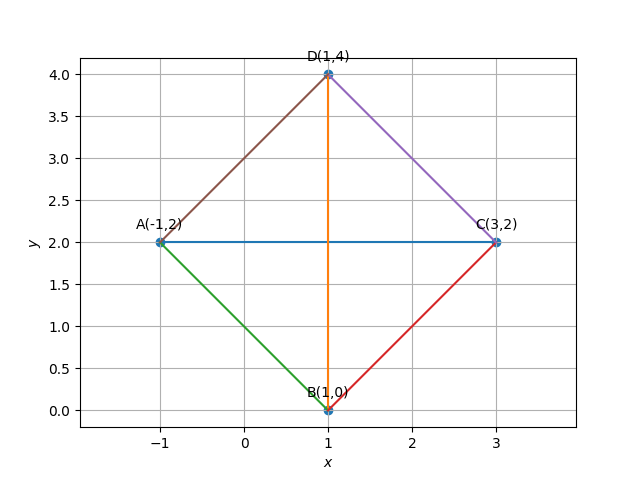
\includegraphics[width=\columnwidth]{chapters/10/7/4/4/figs/square4}
	\end{center}
\caption{}
\label{fig:7/4/4/4Fig5}
\end{figure}
which can also be expressed as
\begin{align}
\vec{B} &= \vec{A} + \vec{P}\myvec{
\vec{e_{1}}&\vec{0}\\
}
\vec{P}^\top \brak{\vec{C}-\vec{A}}\\
\vec{D} &= \vec{A} + \vec{P}\myvec{
\vec{0}&\vec{e_{2}}\\
}
\vec{P}^\top \brak{\vec{C}-\vec{A}}\\
\end{align}
where $\vec{P}$ is the rotation matrix and $\vec{A} \text{ and } \vec{C}$ are the position vectors of opposite vertices.

Derivation of the above formulas:

We know that after shifting the axis and rotating by the required angle any arbitrary square will be aligned with the x and y axis so that we can directly get the vectors $\vec{B} \text{ and } \vec{D}$ as follows
\begin{align}
\vec{C^{\prime\prime}} &= \vec{P}^\top \brak{\vec{C} - \vec{A}}\\
\vec{B^{\prime\prime}} &= \myvec{
\vec{e_{1}} & \vec{0}
}\vec{C^{\prime\prime}} = \myvec{
\vec{e_{1}} & \vec{0}
}\vec{P}^\top \brak{\vec{C} - \vec{A}}\\
\vec{B^{\prime}} &= \vec{P} \vec{B^{\prime\prime}}  = \vec{P}\myvec{
\vec{e_{1}} & \vec{0}
}\vec{P}^\top \brak{\vec{C} - \vec{A}}\\
\vec{B} &= \vec{A}+\vec{B^{\prime}}\\
 &= \vec{A} + \vec{P}\myvec{
\vec{e_{1}}&\vec{0}\\
}
\vec{P}^\top\brak{\vec{C}-\vec{A}}
\end{align}

Similarly for D it can be derived as
\begin{align}
\vec{C^{\prime\prime}} &= \vec{P}^\top \brak{\vec{C} - \vec{A}}\\
\vec{D^{\prime\prime}} &= \myvec{
\vec{0} & \vec{e_{2}}
}\vec{C^{\prime\prime}} = \myvec{
\vec{0} & \vec{e_{2}}
}\vec{P}^\top \brak{\vec{C} - \vec{A}}\\
\vec{D^{\prime}} &= \vec{P} \vec{D^{\prime\prime}} = \vec{P} \myvec{
\vec{0} & \vec{e_{2}}
}\vec{P}^\top \brak{\vec{C} - \vec{A}}\\
\vec{D} &= \vec{A}+\vec{D^{\prime}}\\
 &= \vec{A} + \vec{P}\myvec{
\vec{0}&\vec{e_{2}}\\
}
\vec{P}^\top\brak{\vec{C}-\vec{A}}
\end{align}


Verification of the above formula for the given question

\begin{align}
\vec{B} &= \myvec{
-1\\
2\\
}+\myvec{
\frac{1}{\sqrt{2}} & \frac{1}{\sqrt{2}} \\
-\frac{1}{\sqrt{2}} & \frac{1}{\sqrt{2}}\\
}\myvec{
 1&0\\
 0&0\\
}\myvec{
\frac{1}{\sqrt{2}} & -\frac{1}{\sqrt{2}} \\
\frac{1}{\sqrt{2}} & \frac{1}{\sqrt{2}}\\
}\myvec{
4\\
0\\
}\\
 &= \myvec{
-1\\
2\\
}+\myvec{
\frac{1}{\sqrt{2}} & \frac{1}{\sqrt{2}} \\
-\frac{1}{\sqrt{2}} & \frac{1}{\sqrt{2}}\\
}\myvec{
 1&0\\
 0&0\\
}\myvec{
\frac{4}{\sqrt{2}}\\
\frac{4}{\sqrt{2}}\\
}\\
 &= \myvec{
-1\\
2\\
}+\myvec{
\frac{1}{\sqrt{2}} & \frac{1}{\sqrt{2}} \\
-\frac{1}{\sqrt{2}} & \frac{1}{\sqrt{2}}\\
}\myvec{
\frac{4}{\sqrt{2}}\\
0\\
}\\
 &= \myvec{
-1\\
2\\
}+\myvec{
2\\
-2\\
}\\
 &= \myvec{
1\\
0\\
}\\
\vec{D} &= \myvec{
-1\\
2\\
}+\myvec{
\frac{1}{\sqrt{2}} & \frac{1}{\sqrt{2}} \\
-\frac{1}{\sqrt{2}} & \frac{1}{\sqrt{2}}\\
}\myvec{
 0&0\\
 0&1\\
}\myvec{
\frac{1}{\sqrt{2}} & -\frac{1}{\sqrt{2}} \\
\frac{1}{\sqrt{2}} & \frac{1}{\sqrt{2}}\\
}\myvec{
4\\
0\\
}\\
 &= \myvec{
-1\\
2\\
}+\myvec{
\frac{1}{\sqrt{2}} & \frac{1}{\sqrt{2}} \\
-\frac{1}{\sqrt{2}} & \frac{1}{\sqrt{2}}\\
}\myvec{
 0&0\\
 0&1\\
}\myvec{
\frac{4}{\sqrt{2}}\\
\frac{4}{\sqrt{2}}\\
}\\
 &= \myvec{
-1\\
2\\
}+\myvec{
\frac{1}{\sqrt{2}} & \frac{1}{\sqrt{2}} \\
-\frac{1}{\sqrt{2}} & \frac{1}{\sqrt{2}}\\
}\myvec{
0\\
\frac{4}{\sqrt{2}}\\
}\\
 &= \myvec{
-1\\
2\\
}+\myvec{
2\\
2\\
}\\
 &= \myvec{
1\\
4\\
}
\end{align}
\fi







